\documentclass[14pt,a4paper]{scrartcl}
\usepackage[utf8]{inputenc}
\usepackage[english,russian]{babel}
\usepackage{indentfirst}
\usepackage{misccorr}
\usepackage{graphicx}
\usepackage{amsmath}
\usepackage{textcomp}
\usepackage{alltt}
\usepackage{amssymb}
\usepackage{pgfplots}
\graphicspath{{pictures/}}
\begin{document}
\begin{titlepage}
  \begin{center}
    \large
    МИНИСТЕРСТВО ОБРАЗОВАНИЯ И НАУКИ\\ РОССИЙСКОЙ ФЕДЕРАЦИИ
     
    \vspace{0.5cm}
 
    Федеральное государственное автономное образовательное учреждение высшего образования \\ «МОСКОВСКИЙ ФИЗИКО-ТЕХНИЧЕСКИЙ ИНСТИТУТ (научно-исследовательский институт)»
    \vspace{0.25cm}

	Физтех-школа аэрокосмических технологий
     
    Кафедра общей физики
    \vfill
     
     

    Голубятников Сергей
    \vfill
 
    \textsc{Отчёт по лабораторной работе}\\[5mm]
     
    {\LARGE Исследование эффекта Комптона}
  \bigskip
     
   3 курс, группа Б03-903
\end{center}
\vfill
 
\newlength{\ML}
\settowidth{\ML}{«\underline{\hspace{0.7cm}}» \underline{\hspace{2cm}}}
\hfill
\begin{minipage}{0.4\textwidth}
  Руководитель работы\\
  \underline{\hspace{\ML}} Л.\,В.~Инжечик\\
  «\underline{\hspace{0.7cm}}» \underline{\hspace{2cm}} 2021 г.
\end{minipage}%
\bigskip
 

\vfill
 
\begin{center}
  Долгопрудный, 2021 г.
\end{center}
\end{titlepage}


\tableofcontents
\addcontentsline{exp}{section}{Заголовок добавить в содержание}
\newpage


\section{Цель работы}
С помощью сцинтилляционного спектрометра исследуется энергетический спектр $\gamma$-квантов, рассеянных на графите. Определяется энергия рассеянных $\gamma$-квантов в зависимости от угла рассеяния, а также энергия покоя частиц, на которых происходит комптоновское рассеяние.



\quad  \textbf{В работе используются:} поглотители (свинцовые, алюминивые,железные), коллиматор, сцинтилляционный счётчик, пересчётный прибор, высоковольтный выпрямитель.

\section{Теория}
\quad  Эффект Комптона - увеличение длины волны рассеянного излучения по сравнению с падающим. Интерпретируется как результат упругого соударения $gamma$-квантов и свободных электронов. Запишем для этого процесса законы сохранения энергии и импульса:

\begin{equation}
    mc^2 + \hbar \omega_0 = \gamma mc^2 + \hbar \omega_1
\end{equation}


\begin{equation}
    \frac{\hbar \omega_0}{c} = \gamma mv \mathrm{cos}\phi + \frac{\hbar \omega_1}{c} * \mathrm{cos} \theta
\end{equation}

Решая совместно эти уравнения и переходя от частот к длинам волн, получаем
изменение длины волны рассеянного излучения:

\begin{equation}
    \Delata \lambda = \lambda_1 - \lambda_0 = \frac{h}{mc}(1-\mathrm{cos}\theta) = \Lambda_K (1-\mathrm{cos}\theta) ,
\end{equation}

где $\lambda_0, \lambda_1 $ - длины волн $\gamma$-кванта до и после рассеяния, а величина $\Lambda_K = \frac{h}{mc} = 2.42 \cdot  10 ^{−10}$ см называется комптоновской длиной волны электрона.

\quad При рассении на связанных электронах изменение импульса кванта воспри-
нимается атомом в целом, поэтому набюдается несмещённая компонента в спектре
рассеянного излучения (Томсоновское рассеяние). При увеличении энергии сечение
томсоновского рассеяния уменьшается очень быстро, а сечение комптоновского рассеяния - незначительно. Поэтому эффект Комптона проявляеся наиболее отчётливо
при использовании в качестве рассеивателя легких элементов и при энергии $\gamma$-лучей порядка сотен килоэлектрон-вольт.

\qaud Кроме того, $\gamma$-кванты испытывают в среде поглощение, называемое фотоэффектом и рождением электрон-позитронных пар. Процесс рождения пар пороговый
и по порядку равен 1 МэВ, поэтому в рассматриваемом энергетическом диапазоне
не происходит. При фотоэффекте из атома выбивается электрон, а квант поглощается. Импульс кванта делится между вылетевшим электроном и атомом. Энергия
возбуждения атома обычно поглощается соседними атомами рассеивателя.
\section{Экспериментальная установка}

\quad Схема установки изображена на рисунке 1. Источником излучения служит $^{137}Cs$, помещённый в толстостенный свинцовый контейнер с колиматором. Узкий пучок квантов попадает на графитовую мишень. Рассеянные кванты регистрируются сцинтилляционном счёсчиком. Сцинтиллятором служит кристалл $NaI$.

\begin{center}
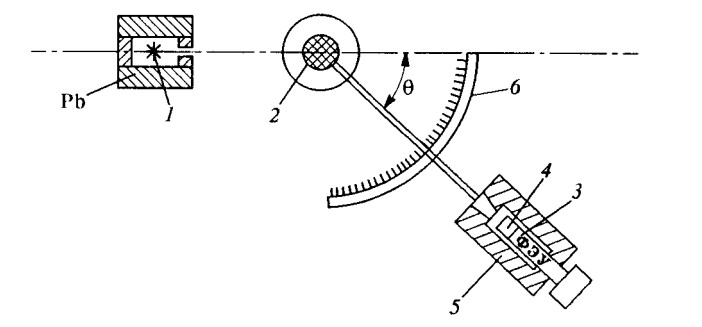
\includegraphics[scale=0.5]{1.png}\newline
\caption{Рис.1. Схема установки. 1 - источник излучения, 2 - графитовая мишень, 3 - ФЭУ, 4 - сцинтиллятор, 5 - свинцовый коллиматор, 6 - лимб }
\end{center}

\section{Ход работы}
Вначале измерим $N(\theta)$ и убедимся, что второй фотопик смещается влево. 

\\
Результаты последовательных измерений приведём в Таблице 1.

\begin{table}[h]
  \centering
  \begin{tabular}{ | c | c | c | c |}
  \hline
  $\theta \degree$ & N & $1 - \cos\theta$ & $\sigma_N$ \\ \hline 
   0 &  900 &  0.000 & 9 \\ \hline
   10 & 925 & 0.015 & 9 \\ \hline
   20 & 904 & 0.060 & 9 \\ \hline
   30 & 706 & 0.134 & 7 \\ \hline
   40 & 690 & 0.234 & 7 \\ \hline
   50 & 614 & 0.357 & 6 \\ \hline
   60 & 569 & 0.500 & 6 \\ \hline
   70 & 503 & 0.657 & 5 \\ \hline
   80 & 452 & 0.826 & 4\\ \hline
   90 & 393 & 0.000 & 4\\ \hline
   100 & 360 & 1.173 & 4\\ \hline
   110 & 339 & 1.341 & 3\\ \hline
   120 & 309 & 1.500 & 3\\ \hline  
  \end{tabular}
  \caption{Результаты измерений}
\end{table}

Погрешности расчитаем по формуле: 

\[\begin{array}{l}
\sigma_{1/N} = \dfrac{\sigma_N}{N^2},\\
\sigma_{1-\cos \theta} = \sin(\theta) \sigma_\theta.\\
\end{array}\]


Оформим полученные величины в виде графика (рис. 2) зависимости $\frac{1}{N}(1-\mathrm{cos}\theta)$.

\begin{center}
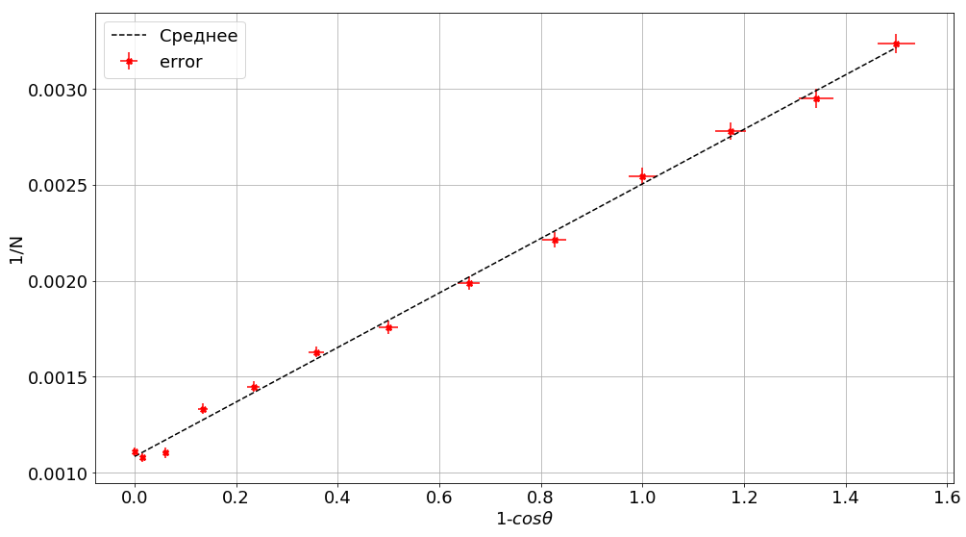
\includegraphics[scale=0.5]{1234.png}\newline
\caption{Рис.2. График зависимости $\frac{1}{N(\theta)}$ от $1-\mathrm{cos}\theta$}
\end{center}










\quad Для того чтобы найти энергию по графику нужно : найти пересечение линии с осью ординат это даст нам значение $N_{best}(0)$. А пересечение линии с прямой $cos \Theta = 0$ даст значение $N_{best}(90)$:

\begin{center}
    $N_{\text{best}}(0) = \dfrac{1}{\frac{1}{N(0)}} = 921 \pm 20$
    
    $N_{\text{best}}(90) = \dfrac{1}{\frac{1}{N(0)}+A} = 399 \pm 7$
    
    \textbf{По графику:} $mc^2 = 506 \pm 20 \text{кЭв} $
\end{center}







где погрешности считались по формулам
\[
\begin{array}{l}
\sigma_{N_{\text{best}}(0)} = \dfrac{\sigma_{\frac{1}{N(0)}}}{(\frac{1}{N(0)})^2},\\[14pt]
\sigma_{N_{\text{best}}(90)} = \dfrac{\sigma_{\frac{1}{N(0)}} + \sigma_{A}}{(\frac{1}{N(0)}+A)^2}.\\
\end{array}
\]

и 

\[\sigma_{mc^2} = \sqrt{ \left( \dfrac{\partial (mc^2)}{\partial N_{\text{наил}}(0)} \right)^2 \sigma_{N_{\text{наил}}(0)}^2 +\left( \dfrac{\partial (mc^2)}{\partial N_{\text{наил}}(90)} \right)^2 \sigma_{N_{\text{наил}}(90)}^2 }\] \\




Результаты вычислений представим в виде таблицы 2.

\begin{table}[h]
    \centering
    \begin{tabular}{|c|c|c|}
    \hline
       Величина  & Значение & Погрешность \\ \hline
        $N_{best}(0)$ & 921 & 20 \\ \hline
        $N_{best}(90)$ & 399 & 7 \\ \hline
        mc$^2$, МэВ & 0.506 & 0.020 \\ \hline
    \end{tabular}
    \caption{Результаты вычислений}
    \label{tab:my_label}
\end{table}



\section{Вывод}
В ходе лабораторной работы исследовали энергетический спект $\gamma - $ квантов, рассеяных на графите. Определили энергию рассеянных $\gamma -$ квантов в зависимости от угла рассеяния, а также энергия покоя частиц, на которых происходит комптоновское рассеяние. Определили энергию рассеянных квантов двумя способами: по формуле ($mc^2 = 0.506$ МэВ) и при помощи графиков ($mc^2 = 0.515$ МэВ). Результаты совпадают с учетом погрешности.


\addcontentsline{toc}{section}{Список используемой литературы}

\newpage

\begin{thebibliography}{}

\bibitem{Sulsky1994}
Лабораторный практикум по общей физике: Учеб. пособие для вузов. Т. 3. Квантовая физика / Игошин Ф.Ф., Самарский Ю.А., Ципенюк Ю.М.; Под ред. Ципенюка Ю.М. - М.:Физматкнига, 2005. 432 стр.



	
\end{thebibliography}

\end{document}
